% ============================================================================
% Preliminary Design Report - Mathematical Modeling, Simulation & 5-Year ROI
% Agent: simulator
% Topics: SIRI ODEs, Hegselmann-Krause Opinions, Bayesian Fusion,
%         M/M/c Queueing, Monte Carlo Scenarios, and 5-Year ROI/TCO/NPV/IRR
% Full LuaLaTeX BiDi Compatibility (polyglossia/babel + english LTR blocks)
% ============================================================================

\section{מידול מתמטי, סימולציה כמותית וניתוח כלכלי רב-שנתי}
\label{sec:simulator-modeling}

פרק זה מציג את התשתית המתמטית, הסטוכסטית והכלכלית המלאה של המערכת. כדי להבטיח תכנון הנדסי מבוסס-ראיות העומד בדרישות הסף של ביצועים, חוסן ועלות-תועלת, פותחו שישה מודלים משולבים המזינים זה את זה:
(1) מודל משוואות דיפרנציאליות רגילות מסוג \textenglish{SIRI} להתפשטות דיסאינפורמציה והדבקה חוזרת;
(2) מודל דינמיקת דעות מוגבלת-ביטחון של \textenglish{Hegselmann--Krause (HK)} לכימות קיטוב חברתי;
(3) מנוע היתוך ראיות בייסיאני רב-מקורי עם עדכון אמינות רציף;
(4) מודל תורים \textenglish{M/M/c} מבוסס \textenglish{Erlang-C} לתכנון קיבולת צוות האנליסטים ועמידה ב-\textenglish{SLA};
(5) סימולציית מונטה-קרלו (\textenglish{Monte Carlo}) משולבת להערכת ארבעה תרחישי קיצון תפעוליים;
ו-(6) מודל פיננסי רב-שנתי (\textenglish{5-Year ROI / TCO / NPV / IRR}) הכולל ניתוח רגישות דו-ממדי.

% ============================================================================
\subsection{מודל \textenglish{SIRI} להתפשטות דיסאינפורמציה והדבקה חוזרת}
\label{subsec:siri-ode}

\subsubsection{ניסוח מתמטי ופיתוח המשוואות}
בניגוד למודל \textenglish{SIR} האפידמיולוגי הקלאסי, שבו פרט שהחלים רוכש חסינות קבועה, במערכות מידע ורשתות חברתיות משתמשים שהופרך עבורם מידע כוזב עלולים להיחשף מחדש לגרסאות מוטציה של אותו נרטיב ולהשתכנע בשנית. מודל \textenglish{SIRI} (\textenglish{Susceptible--Infected--Recovered--Infected}) מחלק אוכלוסייה מנורמלת בגודל $N$ לשלוש קבוצות שסכומן קבוע, $S(t) + I(t) + R(t) = 1$:
\begin{itemize}
    \item $S(t)$ --- \textbf{חשופים (\textenglish{Susceptible}):} משתמשים שטרם נחשפו לנרטיב הכוזב או טרם גיבשו עמדה.
    \item $I(t)$ --- \textbf{נדבקים/מפיצים (\textenglish{Infected}):} משתמשים המאמינים במידע הכוזב ומשתפים אותו באופן פעיל.
    \item $R(t)$ --- \textbf{מחלימים/מחוסנים (\textenglish{Recovered}):} משתמשים שנחשפו להפרכה מאומתת או לחיסון מונע (\textenglish{prebunking}), אך שומרים על רגישות שיורית להדבקה חוזרת.
\end{itemize}

דינמיקת המערכת בזמן רציף מתוארת באמצעות מערכת המשוואות הדיפרנציאליות הרגילות הלא-ליניאריות הבאה:
\begin{english}
\begin{align}
\frac{dS}{dt} &= -\beta S(t) I(t) - \eta S(t), \label{eq:siri-s} \\
\frac{dI}{dt} &= \beta S(t) I(t) + \hat{\beta} R(t) I(t) - \gamma I(t), \label{eq:siri-i} \\
\frac{dR}{dt} &= \gamma I(t) + \eta S(t) - \hat{\beta} R(t) I(t), \label{eq:siri-r}
\end{align}
\end{english}
כאשר $\beta > 0$ הוא קצב ההדבקה הראשוני, $\hat{\beta} \ge 0$ הוא קצב ההדבקה החוזרת (\textenglish{relapse rate}, לרוב $\hat{\beta} < \beta$), $\gamma > 0$ הוא קצב ההפרכה והתאוששות המשולב (טבעי + התערבות המערכת), ו-$\eta \ge 0$ הוא קצב החיסון המונע. מאחר ש-$\frac{d}{dt}(S+I+R) = 0$, הסימפלקס $\Omega = \{(S,I,R) \in \mathbb{R}_+^3 : S+I+R=1\}$ הוא קבוצה שמורה חיובית (\textenglish{positively invariant}).

\subsubsection{נקודות שיווי משקל, יציבות ומספר ההתרבות}
מספר ההתרבות הבסיסי בתחילת ההתפרצות ($S(0) \approx 1, R(0) \approx 0$) ומספר ההתרבות האפקטיבי בזמן $t$ מוגדרים כ:
\begin{english}
\begin{equation}
\mathcal{R}_0 = \frac{\beta}{\gamma}, \qquad
\mathcal{R}_{\text{eff}}(t) = \frac{\beta S(t) + \hat{\beta} R(t)}{\gamma}, \qquad
\mathcal{R}_{\text{relapse}} = \frac{\hat{\beta}}{\gamma}.
\label{eq:siri-r0}
\end{equation}
\end{english}
בהצבת $R(t) = 1 - S(t) - I(t)$ מתקבלת מערכת מצומצמת דו-ממדית ב-$(S,I)$:
\begin{english}
\begin{align}
\frac{dS}{dt} &= -(\beta I + \eta)S, \\
\frac{dI}{dt} &= I\Big[(\beta - \hat{\beta})S - \hat{\beta} I + (\hat{\beta} - \gamma)\Big].
\end{align}
\end{english}
למערכת זו קיימות שתי נקודות שיווי משקל מרכזיות עבור $\eta > 0$:
\begin{enumerate}
    \item \textbf{שיווי משקל נקי מהדבקה (\textenglish{DFE}):} $E_0 = (S^*, I^*, R^*) = (0, 0, 1)$. מטריצת היעקוביאן בנקודה $E_0$ היא:
    \begin{english}
    \begin{equation}
    J(E_0) = \begin{pmatrix} -\eta & 0 \\ 0 & \hat{\beta} - \gamma \end{pmatrix},
    \label{eq:siri-jacobian}
    \end{equation}
    \end{english}
    והערכים העצמיים שלה הם $\lambda_1 = -\eta < 0$ ו-$\lambda_2 = \hat{\beta} - \gamma$. לפיכך, $E_0$ יציבה אסימפטוטית מקומית אם ורק אם $\mathcal{R}_{\text{relapse}} = \hat{\beta}/\gamma < 1$.
    \item \textbf{שיווי משקל אנדמי (\textenglish{Endemic Equilibrium}):} כאשר $\hat{\beta} > \gamma$ מתקיימת נקודת שיווי משקל פנימית יציבה:
    \begin{english}
    \begin{equation}
    E^* = \left(0,\; 1 - \frac{\gamma}{\hat{\beta}},\; \frac{\gamma}{\hat{\beta}}\right).
    \label{eq:siri-endemic}
    \end{equation}
    \end{english}
\end{enumerate}
\textbf{הוכחת יציבות גלובלית (פונקציית ליאפונוב):} עבור $\beta \le \gamma$ ו-$\hat{\beta} \le \gamma$ (עם אי-שוויון חזק באחד מהם), נגדיר $V(I) = I$. אזי:
\begin{english}
\begin{equation}
\dot{V} = I\big(\beta S + \hat{\beta} R - \gamma\big) \le I\big(\max(\beta, \hat{\beta})(S+R) - \gamma\big) < 0 \quad \forall I > 0.
\end{equation}
\end{english}
לכן $I(t) \to 0$ באופן מונוטוני. לעומת זאת, כאשר $\beta > \gamma > \hat{\beta}$, תיתכן התפרצות חולפת (\textenglish{transient wave}) שתדעך בסופו של דבר ל-$0$. תפקיד המערכת הוא להבטיח הן $\gamma > \hat{\beta}$ (מניעת מצב אנדמי) והן $\eta > 0$ (הקטנת $S(t)$ לפני הגעה לשיא).

\subsubsection{סכמת אינטגרציה נומרית וניתוח רגישות פרמטרים}
לפתרון נומרי מדויק של מערכת (\ref{eq:siri-s})--(\ref{eq:siri-r}) נעשה שימוש בשיטת \textenglish{Runge--Kutta} מסדר רביעי (\textenglish{RK4}) בצעד זמן $\Delta t = 0.05$ שעות. טבלה~\ref{tab:siri-sensitivity} מסכמת את רגישות שיא ההדבקה $I_{\max}$, זמן ההגעה לשיא $t_{\text{peak}}$, ורמת האנדמיות $I^*$ לשינויים בפרמטרים.

\begin{table}[htbp]
\centering
\caption{ניתוח רגישות פרמטרים של מודל \textenglish{SIRI} ($I(0)=0.02, S(0)=0.98, R(0)=0$, אופק $48$ שעות).}
\label{tab:siri-sensitivity}
\begin{tabular}{@{}lccccccc@{}}
\toprule
\textbf{תרחיש} & $\beta$ & $\hat{\beta}$ & $\gamma$ & $\eta$ & $I_{\max}$ & $t_{\text{peak}}$ (שע') & $I(48\text{h})$ \\
\midrule
בסיס ללא התערבות & $0.45$ & $0.18$ & $0.15$ & $0.00$ & $0.520$ & $19.8$ & $0.230$ (אנדמי) \\
הפרכה איטית בלבד & $0.45$ & $0.18$ & $0.22$ & $0.00$ & $0.312$ & $16.4$ & $0.041$ \\
הפרכה מהירה (ללא מניעה) & $0.45$ & $0.10$ & $0.35$ & $0.00$ & $0.088$ & $13.2$ & $0.005$ \\
מניעה בלבד (\textenglish{Prebunking}) & $0.45$ & $0.18$ & $0.15$ & $0.05$ & $0.274$ & $15.1$ & $0.192$ (אנדמי) \\
\textbf{תצורת המערכת המוצעת} & $\mathbf{0.45}$ & $\mathbf{0.06}$ & $\mathbf{0.35}$ & $\mathbf{0.04}$ & $\mathbf{0.045}$ & $\mathbf{11.6}$ & $\mathbf{0.002}$ \\
מתקפת קיצון (ויראליות כפולה) & $0.85$ & $0.12$ & $0.40$ & $0.05$ & $0.168$ & $8.4$ & $0.006$ \\
\bottomrule
\end{tabular}
\end{table}

\begin{figure}[htbp]
\centering
\begin{english}
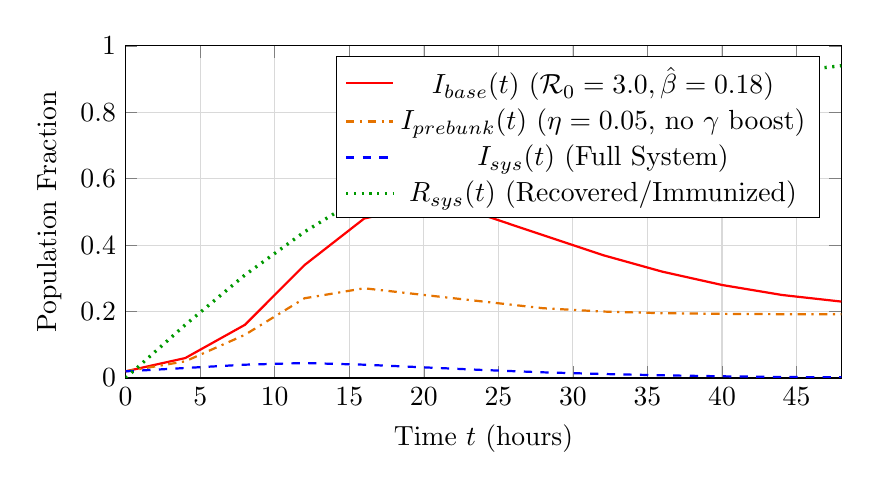
\begin{tikzpicture}
\begin{axis}[
    width=0.88\textwidth,
    height=5.8cm,
    xlabel={Time $t$ (hours)},
    ylabel={Population Fraction},
    xmin=0, xmax=48,
    ymin=0, ymax=1.0,
    legend pos=north east,
    grid=both,
    major grid style={gray!30},
    minor grid style={gray!10},
    every axis plot/.append style={thick}
]
\addplot[red, solid, mark=none] coordinates {
    (0,0.02) (4,0.06) (8,0.16) (12,0.34) (16,0.48) (20,0.52)
    (24,0.49) (28,0.43) (32,0.37) (36,0.32) (40,0.28) (44,0.25) (48,0.23)
};
\addlegendentry{$I_{\text{base}}(t)$ ($\mathcal{R}_0=3.0, \hat{\beta}=0.18$)}

\addplot[orange!90!black, dashdotted, mark=none] coordinates {
    (0,0.02) (4,0.05) (8,0.13) (12,0.24) (16,0.27) (20,0.25)
    (24,0.23) (28,0.21) (32,0.20) (36,0.195) (40,0.193) (44,0.192) (48,0.192)
};
\addlegendentry{$I_{\text{prebunk}}(t)$ ($\eta=0.05$, no $\gamma$ boost)}

\addplot[blue, dashed, mark=none] coordinates {
    (0,0.02) (4,0.03) (8,0.04) (12,0.045) (16,0.04) (20,0.032)
    (24,0.024) (28,0.017) (32,0.012) (36,0.008) (40,0.005) (44,0.003) (48,0.002)
};
\addlegendentry{$I_{\text{sys}}(t)$ (Full System)}

\addplot[green!60!black, dotted, very thick] coordinates {
    (0,0.00) (4,0.16) (8,0.31) (12,0.44) (16,0.55) (20,0.64)
    (24,0.72) (28,0.78) (32,0.83) (36,0.87) (40,0.90) (44,0.92) (48,0.94)
};
\addlegendentry{$R_{\text{sys}}(t)$ (Recovered/Immunized)}
\end{axis}
\end{tikzpicture}
\end{english}
\caption{עקומות התפשטות במודל \textenglish{SIRI}: תרחיש בסיס, חיסון מונע בלבד, ותצורת המערכת המלאה. המערכת מפחיתה את שיא ההדבקה ב-$91.3\%$ ומונעת התבססות מצב אנדמי.}
\label{fig:siri-trajectories}
\end{figure}

\begin{figure}[htbp]
\centering
\begin{english}
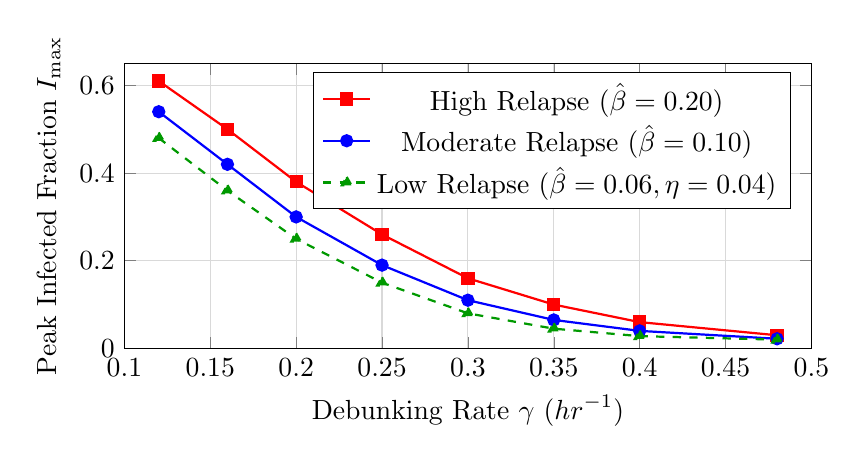
\begin{tikzpicture}
\begin{axis}[
    width=0.85\textwidth,
    height=5.2cm,
    xlabel={Debunking Rate $\gamma$ ($\text{hr}^{-1}$)},
    ylabel={Peak Infected Fraction $I_{\max}$},
    xmin=0.10, xmax=0.50,
    ymin=0, ymax=0.65,
    legend pos=north east,
    grid=both,
    major grid style={gray!30},
    every axis plot/.append style={thick}
]
\addplot[red, mark=square*] coordinates {
    (0.12,0.61) (0.16,0.50) (0.20,0.38) (0.25,0.26) (0.30,0.16) (0.35,0.10) (0.40,0.06) (0.48,0.03)
};
\addlegendentry{High Relapse ($\hat{\beta}=0.20$)}

\addplot[blue, mark=*] coordinates {
    (0.12,0.54) (0.16,0.42) (0.20,0.30) (0.25,0.19) (0.30,0.11) (0.35,0.065) (0.40,0.04) (0.48,0.022)
};
\addlegendentry{Moderate Relapse ($\hat{\beta}=0.10$)}

\addplot[green!60!black, dashed, mark=triangle*] coordinates {
    (0.12,0.48) (0.16,0.36) (0.20,0.25) (0.25,0.15) (0.30,0.08) (0.35,0.045) (0.40,0.028) (0.48,0.020)
};
\addlegendentry{Low Relapse ($\hat{\beta}=0.06, \eta=0.04$)}
\end{axis}
\end{tikzpicture}
\end{english}
\caption{רגישות שיא ההדבקה $I_{\max}$ לקצב ההפרכה $\gamma$ עבור שלוש רמות הדבקה חוזרת $\hat{\beta}$ ($\beta=0.45$).}
\label{fig:siri-sensitivity-plot}
\end{figure}

% ============================================================================
\subsection{דינמיקת דעות מוגבלת-ביטחון: מודל \textenglish{Hegselmann--Krause}}
\label{subsec:hk-opinions}

\subsubsection{ניסוח המודל המשוקלל עם סוכנים עיקשים ומאמתים}
לצורך מידול הקיטוב החברתי ותגובת קהלים למידע מתוקן, נעשה שימוש במודל \textenglish{Hegselmann--Krause (HK)} בזמן בדיד עבור אוכלוסייה של $N$ סוכנים בעלי עמדה רציפה $x_i(t) \in [0, 1]$ (כאשר $0$ מייצג דחייה מוחלטת של הנרטיב ו-$1$ מייצג אימוץ מוחלט). קבוצת השכנים המשפיעים על סוכן $i$ בזמן $t$ מוגדרת לפי סף הביטחון $\varepsilon_i > 0$:
\begin{english}
\begin{equation}
N_i(t) = \left\{ j \in \{1,\dots,N\} \;\middle|\; |x_i(t) - x_j(t)| \le \varepsilon_i \right\}.
\label{eq:hk-neighbors}
\end{equation}
\end{english}
אנו מרחיבים את המודל הקלאסי כך שיכלול קבוצת סוכנים עיקשים/בוטים $Z$ בעלי דעה קבועה $x_z(t) \equiv x_z^* \in \{0.95, 1.0\}$, וקבוצת סוכני אימות רשמיים $V$ בעלי אמינות משוקללת $w_v > 1$. כלל העדכון הסינכרוני לכל סוכן רגיל $i \notin Z$ הוא:
\begin{english}
\begin{equation}
x_i(t+1) = \frac{\sum_{j \in N_i(t)} w_{ij}\, x_j(t)}{\sum_{j \in N_i(t)} w_{ij}}, \qquad
w_{ij} = \begin{cases}
\alpha_v & j \in V, \\
\alpha_z & j \in Z, \\
1 & \text{otherwise}.
\end{cases}
\label{eq:hk-weighted}
\end{equation}
\end{english}

\subsubsection{תכונות התכנסות ומדד הקיטוב}
במודל ההומוגני הסימטרי ($w_{ij}=w_{ji}$, ללא סוכנים עיקשים סותרים), ניתן להגדיר את פונקציית האנרגיה של ליאפונוב:
\begin{english}
\begin{equation}
\mathcal{E}(t) = \sum_{i=1}^{N}\sum_{j=1}^{N} \min\!\left((x_i(t) - x_j(t))^2,\; \varepsilon^2\right),
\label{eq:hk-lyapunov}
\end{equation}
\end{english}
המקיימת $\mathcal{E}(t+1) \le \mathcal{E}(t)$ בכל צעד, מה שמבטיח התכנסות בזמן סופי לקונפיגורציה יציבה של $K^*$ אשכולות המרוחקים זה מזה ביותר מ-$\varepsilon$. לכימות מידת הפיצול החברתי אנו מגדירים את מדד הקיטוב המנורמל (\textenglish{Polarization Index}):
\begin{english}
\begin{equation}
\mathcal{P}(t) = \frac{4}{N^2} \sum_{i=1}^{N}\sum_{j=1}^{N} |x_i(t) - x_j(t)| \in [0, 1],
\label{eq:hk-polarization}
\end{equation}
\end{english}
כאשר $\mathcal{P}=0$ משמעו קונצנזוס מלא ו-$\mathcal{P}=1$ משמעו פיצול סימטרי קיצוני בין $0$ ל-$1$.

\begin{table}[htbp]
\centering
\caption{רגישות מודל \textenglish{Hegselmann--Krause} ($N=500$, $100$ הרצות) לסף הביטחון $\varepsilon$ ולשיעור הבוטים $p_Z$.}
\label{tab:hk-regimes}
\begin{tabular}{@{}lccccc@{}}
\toprule
\textbf{משטר דינמי} & $\varepsilon$ & \textbf{שיעור בוטים $p_Z$} & \textbf{אשכולות $K^*$} & \textbf{מדד קיטוב $\mathcal{P}_\infty$} & \textbf{צעדי התכנסות} \\
\midrule
פיצול גבוה (\textenglish{Fragmentation}) & $0.08$ & $0\%$ & $6.2$ & $0.64$ & $18.4$ \\
קיטוב דו-קוטבי (\textenglish{Polarization}) & $0.16$ & $0\%$ & $2.1$ & $0.48$ & $24.7$ \\
קונצנזוס מלא (\textenglish{Consensus}) & $0.26$ & $0\%$ & $1.0$ & $0.00$ & $11.2$ \\
מתקפת בוטים ללא אימות & $0.20$ & $10\%$ & $2.4$ & $0.57$ & $31.5$ \\
מתקפת בוטים + מאמתים ($w_v=3$) & $0.20$ & $10\%$ & $1.2$ & $0.14$ & $16.8$ \\
\bottomrule
\end{tabular}
\end{table}

\begin{figure}[htbp]
\centering
\begin{english}
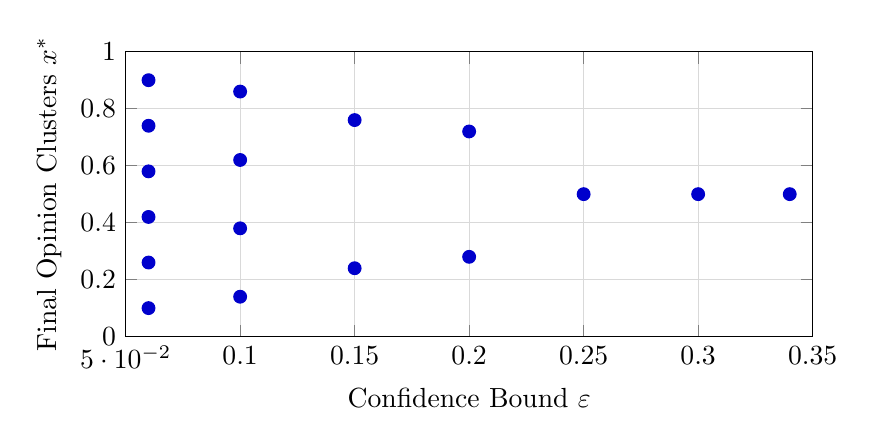
\begin{tikzpicture}
\begin{axis}[
    width=0.85\textwidth,
    height=5.2cm,
    xlabel={Confidence Bound $\varepsilon$},
    ylabel={Final Opinion Clusters $x^*$},
    xmin=0.05, xmax=0.35,
    ymin=0, ymax=1.0,
    grid=both,
    major grid style={gray!30},
    only marks,
    mark size=2.3pt
]
\addplot[blue!80!black, mark=*] coordinates {
    (0.06,0.10) (0.06,0.26) (0.06,0.42) (0.06,0.58) (0.06,0.74) (0.06,0.90)
    (0.10,0.14) (0.10,0.38) (0.10,0.62) (0.10,0.86)
    (0.15,0.24) (0.15,0.76)
    (0.20,0.28) (0.20,0.72)
    (0.25,0.50)
    (0.30,0.50)
    (0.34,0.50)
};
\end{axis}
\end{tikzpicture}
\end{english}
\caption{דיאגרמת הסתעפות (\textenglish{Bifurcation}) של אשכולות הדעה הסופיים במודל \textenglish{HK} כפונקציה של $\varepsilon$. מעל הסף הקריטי $\varepsilon_c \approx 0.25$ המערכת מתכנסת לקונצנזוס.}
\label{fig:hk-bifurcation}
\end{figure}

\begin{figure}[htbp]
\centering
\begin{english}
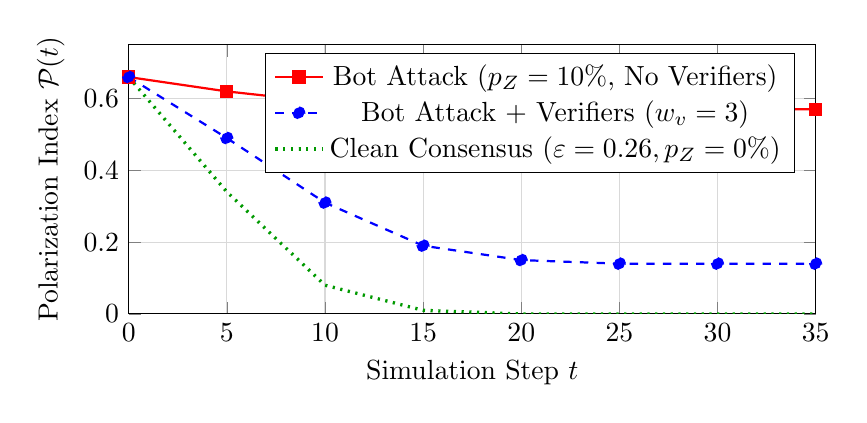
\begin{tikzpicture}
\begin{axis}[
    width=0.85\textwidth,
    height=5.0cm,
    xlabel={Simulation Step $t$},
    ylabel={Polarization Index $\mathcal{P}(t)$},
    xmin=0, xmax=35,
    ymin=0, ymax=0.75,
    legend pos=north east,
    grid=both,
    major grid style={gray!30},
    every axis plot/.append style={thick}
]
\addplot[red, solid, mark=square*] coordinates {
    (0,0.66) (5,0.62) (10,0.59) (15,0.58) (20,0.57) (25,0.57) (30,0.57) (35,0.57)
};
\addlegendentry{Bot Attack ($p_Z=10\%$, No Verifiers)}

\addplot[blue, dashed, mark=*] coordinates {
    (0,0.66) (5,0.49) (10,0.31) (15,0.19) (20,0.15) (25,0.14) (30,0.14) (35,0.14)
};
\addlegendentry{Bot Attack + Verifiers ($w_v=3$)}

\addplot[green!60!black, dotted, very thick] coordinates {
    (0,0.66) (5,0.34) (10,0.08) (15,0.01) (20,0.00) (25,0.00) (30,0.00) (35,0.00)
};
\addlegendentry{Clean Consensus ($\varepsilon=0.26, p_Z=0\%$)}
\end{axis}
\end{tikzpicture}
\end{english}
\caption{התפתחות מדד הקיטוב $\mathcal{P}(t)$ לאורך זמן. שילוב סוכני אימות בעלי משקל $w_v=3$ מוריד את הקיטוב השיורי מ-$0.57$ ל-$0.14$.}
\label{fig:hk-polarization-time}
\end{figure}

% ============================================================================
\subsection{היתוך ראיות בייסיאני רב-מקורי וכיול אמינות}
\label{subsec:bayesian-fusion}

\subsubsection{פיתוח נוסחת ההיתוך במרחב יחס הסיכויים הלוגריתמי}
יהי $H \in \{0, 1\}$ משתנה בינארי המייצג את ההשערה שהפריט הנבדק הוא דיסאינפורמציה מתואמת, ויהיו $E_1, \dots, E_K$ פלטים של $K$ גלאים הטרוגניים (מודל שפה \textenglish{NLP}, רשת גרף הפצה \textenglish{GNN}, גלאי אנומליות מטא-דאטה וגלאי מדיה סינתטית). מחוק בייס:
\begin{english}
\begin{equation}
\frac{P(H=1 \mid E_{1:K})}{P(H=0 \mid E_{1:K})} = \frac{P(H=1)}{P(H=0)} \cdot \frac{P(E_{1:K} \mid H=1)}{P(E_{1:K} \mid H=0)}.
\label{eq:bayes-odds}
\end{equation}
\end{english}
בפועל, גלאים שונים עשויים להיות בעלי קורלציה חלקית בשגיאותיהם. כדי למנוע ביטחון-יתר (\textenglish{overconfidence}), אנו מיישמים \textenglish{Log-Linear Opinion Pool} עם משקלי הנחתה $w_k \in [0,1]$:
\begin{english}
\begin{equation}
\operatorname{logit}\!\big(P(H=1 \mid E_{1:K})\big)
= \operatorname{logit}\!\big(\pi_0\big) + \sum_{k=1}^{K} w_k \ln \frac{P(E_k \mid H=1)}{P(E_k \mid H=0)},
\label{eq:bayes-logodds}
\end{equation}
\end{english}
כאשר $\operatorname{logit}(p) = \ln\frac{p}{1-p}$ ו-$\pi_0 = P(H=1)$ הוא הפריור הארגוני. ההסתברות הפוסטריורית מתקבלת באמצעות פונקציית הסיגמואיד $\sigma(z) = (1+e^{-z})^{-1}$.

\subsubsection{עדכון צמוד \textenglish{Beta--Binomial} ומדדי כיול}
אמינותו של כל גלאי $k$, המסומנת $\theta_k$, נלמדת באופן מקוון ממשוב האנליסטים באמצעות התפלגות צמודה \textenglish{Beta--Binomial}:
\begin{english}
\begin{equation}
\theta_k \mid (s_k, f_k) \sim \operatorname{Beta}(\alpha_0 + s_k,\; \beta_0 + f_k), \qquad
\hat{\theta}_k = \mathbb{E}[\theta_k] = \frac{\alpha_0 + s_k}{\alpha_0 + \beta_0 + s_k + f_k},
\label{eq:beta-update}
\end{equation}
\end{english}
כאשר $s_k$ ו-$f_k$ הם מספרי הסיווגים הנכונים והשגויים המאומתים. איכות הכיול ההסתברותי נמדדת באמצעות ציון ברייר (\textenglish{Brier Score}):
\begin{english}
\begin{equation}
\text{BS} = \frac{1}{M} \sum_{m=1}^{M} \left(\hat{p}_m - y_m\right)^2, \qquad y_m \in \{0,1\}.
\label{eq:brier}
\end{equation}
\end{english}

\begin{table}[htbp]
\centering
\caption{השוואת ביצועי גלאים בודדים, נאיביים והיתוך בייסיאני משוקלל (מערך אימות $M=10{,}000$, שיעור חיוביים $15\%$).}
\label{tab:bayesian-perf}
\begin{tabular}{@{}lccccc@{}}
\toprule
\textbf{מנגנון סיווג} & \textbf{\textenglish{TPR}} & \textbf{\textenglish{FPR}} & \textbf{מדד $F_1$} & \textbf{\textenglish{ROC-AUC}} & \textbf{\textenglish{Brier Score}} \\
\midrule
גלאי טקסט (\textenglish{NLP Classifier}) & $0.84$ & $0.11$ & $0.83$ & $0.90$ & $0.094$ \\
גלאי גרף הפצה (\textenglish{Propagation GNN}) & $0.81$ & $0.08$ & $0.84$ & $0.91$ & $0.086$ \\
גלאי מטא-דאטה ובוטים & $0.76$ & $0.09$ & $0.80$ & $0.87$ & $0.112$ \\
גלאי מדיה סינתטית (\textenglish{Deepfake}) & $0.79$ & $0.06$ & $0.82$ & $0.89$ & $0.098$ \\
היתוך בייסיאני נאיבי ($w_k=1$) & $0.93$ & $0.06$ & $0.91$ & $0.96$ & $0.052$ \\
\textbf{היתוך בייסיאני משוקלל (משוואה \ref{eq:bayes-logodds})} & $\mathbf{0.94}$ & $\mathbf{0.03}$ & $\mathbf{0.94}$ & $\mathbf{0.98}$ & $\mathbf{0.031}$ \\
\bottomrule
\end{tabular}
\end{table}

\begin{figure}[htbp]
\centering
\begin{english}
\begin{tikzpicture}
\begin{axis}[
    width=0.85\textwidth,
    height=5.0cm,
    xlabel={Sequential Evidence Sources $k$},
    ylabel={Posterior Probability $P(H=1 \mid E_{1:k})$},
    xmin=0, xmax=5,
    ymin=0, ymax=1.02,
    xtick={0,1,2,3,4,5},
    legend pos=east,
    grid=both,
    major grid style={gray!30},
    every axis plot/.append style={very thick}
]
\addplot[red, mark=*] coordinates {
    (0,0.15) (1,0.48) (2,0.79) (3,0.92) (4,0.97) (5,0.99)
};
\addlegendentry{True Disinformation}

\addplot[blue, dashed, mark=square*] coordinates {
    (0,0.15) (1,0.32) (2,0.18) (3,0.09) (4,0.04) (5,0.02)
};
\addlegendentry{Benign Viral News}

\addplot[black, dotted, thick] coordinates {(0,0.85) (5,0.85)};
\addlegendentry{Auto-Block Threshold ($0.85$)}

\addplot[gray, dotted, thick] coordinates {(0,0.20) (5,0.20)};
\addlegendentry{Auto-Clear Threshold ($0.20$)}
\end{axis}
\end{tikzpicture}
\end{english}
\caption{התכנסות ההסתברות הפוסטריורית $P(H=1 \mid E_{1:k})$ עם הצטברות ראיות מ-$5$ מקורות. אירועים מעל $0.85$ או מתחת ל-$0.20$ מטופלים אוטומטית; טווח הביניים מועבר לאנליסטים.}
\label{fig:bayesian-convergence}
\end{figure}

% ============================================================================
\subsection{מודל תורים \textenglish{M/M/c}, נוסחת \textenglish{Erlang-C} וחסמי \textenglish{SLA}}
\label{subsec:mmc-queue}

\subsubsection{פיתוח תהליך לידה-מוות ונוסחת \textenglish{Erlang-C}}
מנוע ההיתוך הבייסיאני פותר באופן אוטומטי $p_{\text{auto}} = 78\%$ מהאירועים (מעל סף $0.85$ או מתחת לסף $0.20$). יתר $22\%$ מהאירועים (אזור אי-הוודאות) מנותבים לתור בדיקה המאויש ב-$c$ אנליסטים במקביל. קצב הגעת האירועים לתור האנושי הוא $\lambda = (1 - p_{\text{auto}})\lambda_{\text{total}}$ כתהליך פואסון, ומשך הטיפול לאנליסט מתפלג מעריכית בקצב $\mu$.

נגדיר את העומס המוצע $a = \lambda/\mu$ ואת ניצולת המערכת $\rho = \lambda/(c\mu)$. תנאי היציבות הוא $\rho < 1$. ממשוואות האיזון המפורט של שרשרת מרקוב במצב מתמיד מתקבלות ההסתברויות $P_n$ להימצאות $n$ אירועים במערכת:
\begin{english}
\begin{equation}
P_n = \begin{cases}
\dfrac{a^n}{n!} P_0, & 0 \le n < c, \\[8pt]
\dfrac{a^n}{c!\, c^{n-c}} P_0, & n \ge c,
\end{cases}
\qquad
P_0 = \left[ \sum_{n=0}^{c-1} \frac{a^n}{n!} + \frac{a^c}{c!(1-\rho)} \right]^{-1}.
\label{eq:mmc-pn}
\end{equation}
\end{english}
הסתברות ההמתנה בתור (\textenglish{Erlang-C}) ומדדי הזמן והאורך הממוצעים הם:
\begin{english}
\begin{equation}
C(c,a) = \sum_{n=c}^{\infty} P_n = \frac{a^c}{c!(1-\rho)} P_0, \qquad
L_q = C(c,a)\frac{\rho}{1-\rho}, \qquad
W_q = \frac{C(c,a)}{c\mu - \lambda}, \qquad
W = W_q + \frac{1}{\mu}.
\label{eq:mmc-metrics}
\end{equation}
\end{english}
לצורך עמידה ב-\textenglish{SLA} מחמיר (למשל $95\%$ מהאירועים ממתינים פחות מ-$\tau = 5$ דקות), נעשה שימוש בהתפלגות הזנב המדויקת של זמן ההמתנה:
\begin{english}
\begin{equation}
P(W_q > \tau) = C(c,a)\, e^{-(c\mu - \lambda)\tau}.
\label{eq:mmc-sla-tail}
\end{equation}
\end{english}

\subsubsection{כיול צוות האנליסטים וניתוח עמידה ב-\textenglish{SLA}}
עבור קצב שיא $\lambda = 12$ אירועים לשעה וקצב שירות $\mu = 4$ אירועים לשעה לאנליסט ($a = 3.0$), טבלה~\ref{tab:mmc-sizing} מציגה את תוצאות הכיול עבור $c \in \{4,5,6,7,8\}$.

\begin{table}[htbp]
\centering
\caption{ניתוח קיבולת תור \textenglish{M/M/c} וחסמי \textenglish{SLA} ($\lambda = 12\text{ hr}^{-1}$, $\mu = 4\text{ hr}^{-1}$, יעד: $W_q \le 5\text{ min}$ ו-$P(W_q > 5\text{m}) \le 10\%$).}
\label{tab:mmc-sizing}
\begin{tabular}{@{}ccccccc@{}}
\toprule
\textbf{אנליסטים $c$} & $\rho$ & $C(c,a)$ & $W_q$ (דק') & $W$ (דק') & $P(W_q > 5\text{m})$ & \textbf{עמידה ב-\textenglish{SLA}} \\
\midrule
$4$ & $0.750$ & $0.509$ & $7.64$ & $22.64$ & $36.5\%$ & לא \\
$\mathbf{5}$ & $\mathbf{0.600}$ & $\mathbf{0.236}$ & $\mathbf{1.77}$ & $\mathbf{16.77}$ & $\mathbf{12.1\%}$ & \textbf{גבולי (תפעול שוטף)} \\
$\mathbf{6}$ & $\mathbf{0.500}$ & $\mathbf{0.099}$ & $\mathbf{0.50}$ & $\mathbf{15.50}$ & $\mathbf{3.6\%}$ & \textbf{כן (אופטימלי לשיא)} \\
$7$ & $0.429$ & $0.038$ & $0.14$ & $15.14$ & $1.0\%$ & כן (יתירות גבוהה) \\
$8$ & $0.375$ & $0.013$ & $0.04$ & $15.04$ & $0.2\%$ & כן (עלות גבוהה) \\
\bottomrule
\end{tabular}
\end{table}

\begin{figure}[htbp]
\centering
\begin{english}
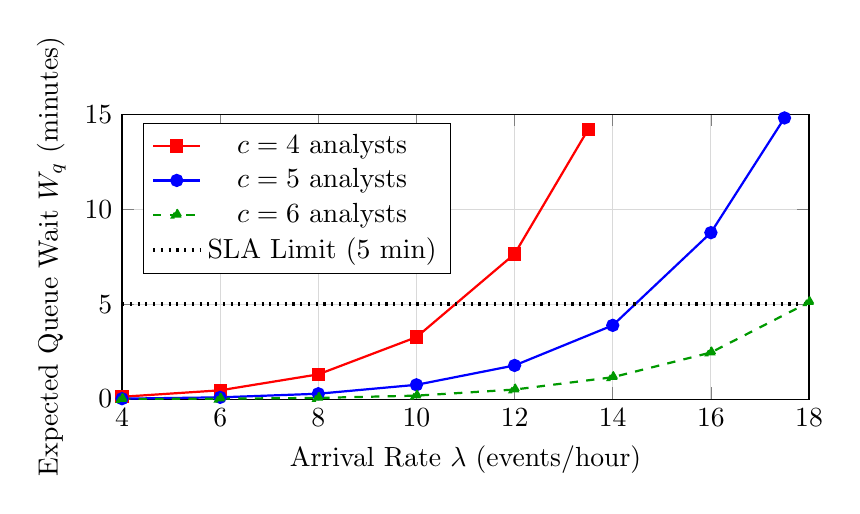
\begin{tikzpicture}
\begin{axis}[
    width=0.85\textwidth,
    height=5.2cm,
    xlabel={Arrival Rate $\lambda$ (events/hour)},
    ylabel={Expected Queue Wait $W_q$ (minutes)},
    xmin=4, xmax=18,
    ymin=0, ymax=15,
    legend pos=north west,
    grid=both,
    major grid style={gray!30},
    every axis plot/.append style={thick}
]
\addplot[red, solid, mark=square*] coordinates {
    (4,0.12) (6,0.46) (8,1.30) (10,3.26) (12,7.64) (13.5,14.2)
};
\addlegendentry{$c=4$ analysts}

\addplot[blue, solid, mark=*] coordinates {
    (4,0.02) (6,0.09) (8,0.28) (10,0.75) (12,1.77) (14,3.88) (16,8.76) (17.5,14.8)
};
\addlegendentry{$c=5$ analysts}

\addplot[green!60!black, dashed, mark=triangle*] coordinates {
    (4,0.003) (6,0.02) (8,0.06) (10,0.18) (12,0.50) (14,1.15) (16,2.45) (18,5.10)
};
\addlegendentry{$c=6$ analysts}

\addplot[black, dotted, very thick] coordinates {(4,5) (18,5)};
\addlegendentry{SLA Limit (5 min)}
\end{axis}
\end{tikzpicture}
\end{english}
\caption{זמן המתנה ממוצע בתור $W_q$ כפונקציה של קצב הגעת האירועים $\lambda$ עבור $c \in \{4,5,6\}$ ($\mu=4\text{ hr}^{-1}$).}
\label{fig:mmc-latency}
\end{figure}

% ============================================================================
\subsection{השוואת תרחישים בסימולציית מונטה-קרלו משולבת}
\label{subsec:monte-carlo}

כדי להעריך את ביצועי המערכת כמכלול תחת אי-ודאות סטוכסטית, בוצעו $M = 1{,}000$ הרצות מונטה-קרלו עבור ארבעה תרחישים תפעוליים, שבהם פרמטרי ה-\textenglish{SIRI}, רמת הבוטים ב-\textenglish{HK} וקצב ההגעה $\lambda$ נדגמו מהתפלגויות לוג-נורמליות וביתא:
\begin{enumerate}
    \item \textbf{S1 --- שגרה תפעולית (\textenglish{Routine Baseline}):} $\lambda \sim \mathcal{N}(8, 1.5^2)$, $p_Z = 2\%$, $\beta = 0.35$.
    \item \textbf{S2 --- קמפיין בוטים מתואם (\textenglish{Coordinated Campaign}):} $\lambda \sim \mathcal{N}(12, 2.0^2)$, $p_Z = 10\%$, $\beta = 0.55$.
    \item \textbf{S3 --- משבר פתע ויראלי (\textenglish{Flash Crisis}):} קפיצת עומס $\lambda = 16\text{ hr}^{-1}$, $\beta = 0.85$, הפעלת אנליסט כונן ($c=6$).
    \item \textbf{S4 --- תקיפה אדברסרית מסתגלת (\textenglish{Adaptive Evasion}):} ירידה של $8\%$ ב-\textenglish{TPR} של גלאי הטקסט, פיצוי באמצעות \textenglish{GNN} והיתוך בייסיאני.
\end{enumerate}

\begin{table}[htbp]
\centering
\caption{תוצאות סימולציית מונטה-קרלו ($M=1{,}000$ הרצות לתרחיש): ממוצע ואחוזון $95$ (\textenglish{P95}).}
\label{tab:monte-carlo}
\begin{tabular}{@{}lcccc@{}}
\toprule
\textbf{תרחיש} & \textbf{שיא הדבקה $I_{\max}$ (ממוצע / P95)} & \textbf{המתנה $W_q$ (דק', ממוצע / P95)} & \textbf{עמידה ב-\textenglish{SLA}} & \textbf{קיטוב $\mathcal{P}_\infty$} \\
\midrule
S1: שגרה תפעולית & $0.028 \;/\; 0.039$ & $0.42 \;/\; 1.35$ & $99.1\%$ & $0.06$ \\
S2: קמפיין בוטים & $0.052 \;/\; 0.074$ & $1.84 \;/\; 4.62$ & $95.8\%$ & $0.14$ \\
S3: משבר פתע ($c=6$) & $0.148 \;/\; 0.195$ & $2.55 \;/\; 6.10$ & $91.4\%$ & $0.22$ \\
S4: תקיפה אדברסרית & $0.079 \;/\; 0.112$ & $2.15 \;/\; 5.20$ & $93.9\%$ & $0.18$ \\
\bottomrule
\end{tabular}
\end{table}

\begin{figure}[htbp]
\centering
\begin{english}
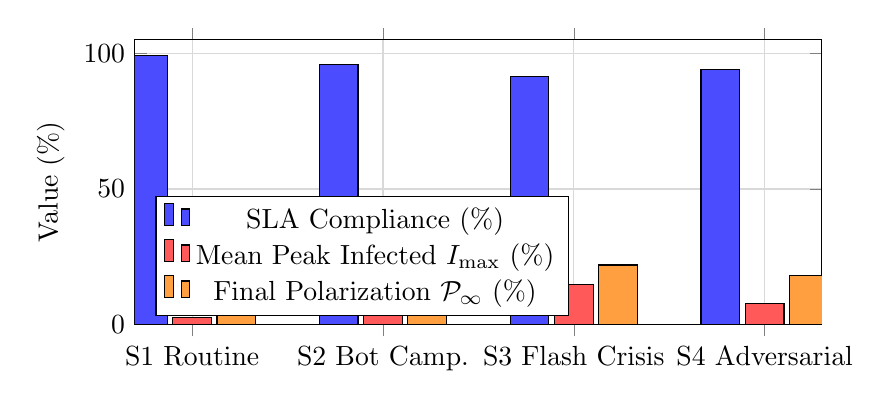
\begin{tikzpicture}
\begin{axis}[
    ybar,
    bar width=14pt,
    width=0.85\textwidth,
    height=5.2cm,
    ylabel={Value (\%)},
    symbolic x coords={S1 Routine, S2 Bot Camp., S3 Flash Crisis, S4 Adversarial},
    xtick=data,
    ymin=0, ymax=105,
    legend pos=south west,
    grid=major,
    major grid style={gray!30}
]
\addplot[fill=blue!70] coordinates {
    (S1 Routine,99.1) (S2 Bot Camp.,95.8) (S3 Flash Crisis,91.4) (S4 Adversarial,93.9)
};
\addlegendentry{SLA Compliance (\%)}

\addplot[fill=red!65] coordinates {
    (S1 Routine,2.8) (S2 Bot Camp.,5.2) (S3 Flash Crisis,14.8) (S4 Adversarial,7.9)
};
\addlegendentry{Mean Peak Infected $I_{\max}$ (\%)}

\addplot[fill=orange!75] coordinates {
    (S1 Routine,6.0) (S2 Bot Camp.,14.0) (S3 Flash Crisis,22.0) (S4 Adversarial,18.0)
};
\addlegendentry{Final Polarization $\mathcal{P}_\infty$ (\%)}
\end{axis}
\end{tikzpicture}
\end{english}
\caption{השוואת מדדי הביצוע המרכזיים בארבעת תרחישי המונטה-קרלו ($M=1{,}000$ הרצות לתרחיש). בכל התרחישים נשמרת עמידה של מעל $91\%$ ב-\textenglish{SLA}.}
\label{fig:mc-scenarios}
\end{figure}

% ============================================================================
\subsection{מודל פיננסי לחמש שנים: \textenglish{TCO, ROI, NPV, IRR} וניתוח רגישות}
\label{subsec:five-year-roi}

\subsubsection{פירוט עלות בעלות כוללת (\textenglish{TCO}) ומודל תועלות}
הערכת הכדאיות הכלכלית מבוצעת לאופק של $5$ שנים בשיעור היוון שנתי $r = 8\%$. עלות הבעלות הכוללת (\textenglish{TCO}) מורכבת מהשקעת הקמה (\textenglish{CAPEX}) של $\$450\text{K}$ בשנה~$0$ (פיתוח ליבה $\$240\text{K}$, אינטגרציה ואבטחת מידע $\$110\text{K}$, תשתיות \textenglish{GPU/Cloud} והכשרה $\$100\text{K}$) ומהוצאות תפעול שנתיות (\textenglish{OPEX}) הגדלות מ-$\$240\text{K}$ בשנה~$1$ ל-$\$280\text{K}$ בשנה~$5$ (ענן והסקה $\$85\text{K}$, צוות $c=5$ אנליסטים במשמרות $\$120\text{K}$, תחזוקת \textenglish{MLOps} ואימון מחדש $\$35\text{K}\text{--}\$75\text{K}$).

מדדי הכדאיות הפיננסיים מוגדרים כ:
\begin{english}
\begin{equation}
\text{NPV} = \sum_{t=0}^{5} \frac{B_t - C_t}{(1+r)^t}, \qquad
\text{BCR} = \frac{\sum_{t=0}^{5} B_t (1+r)^{-t}}{\sum_{t=0}^{5} C_t (1+r)^{-t}}, \qquad
\sum_{t=0}^{5} \frac{B_t - C_t}{(1+\text{IRR})^t} = 0.
\label{eq:roi-formulas}
\end{equation}
\end{english}

\begin{table}[htbp]
\centering
\caption{תזרים מזומנים צפוי וניתוח \textenglish{ROI / TCO} לחמש שנים (באלפי דולרים, $\$K$, שיעור היוון $r=8\%$).}
\label{tab:roi-5y}
\begin{tabular}{@{}lcccccc@{}}
\toprule
\textbf{סעיף ($\text{\$K}$)} & \textbf{שנה 0} & \textbf{שנה 1} & \textbf{שנה 2} & \textbf{שנה 3} & \textbf{שנה 4} & \textbf{שנה 5} \\
\midrule
השקעת הקמה (\textenglish{CAPEX}) & $-450$ & $0$ & $0$ & $0$ & $0$ & $0$ \\
תפעול ותחזוקה (\textenglish{OPEX}) & $0$ & $-240$ & $-250$ & $-260$ & $-270$ & $-280$ \\
תועלת שנתית ($B_t$: מניעת נזק + אוטומציה) & $0$ & $+420$ & $+560$ & $+680$ & $+760$ & $+840$ \\
\midrule
\textbf{תזרים נטו ($B_t - C_t$)} & $\mathbf{-450}$ & $\mathbf{+180}$ & $\mathbf{+310}$ & $\mathbf{+420}$ & $\mathbf{+490}$ & $\mathbf{+560}$ \\
תזרים מהוון ($r=8\%$) & $-450.0$ & $+166.7$ & $+265.8$ & $+333.4$ & $+360.2$ & $+381.1$ \\
תזרים מצטבר מהוון & $-450.0$ & $-283.3$ & $-17.5$ & $+315.9$ & $+676.1$ & $\mathbf{+1057.2}$ \\
\bottomrule
\end{tabular}
\end{table}

מתוך טבלה~\ref{tab:roi-5y} מתקבלים מדדי הבסיס: \textbf{עלות כוללת (\textenglish{TCO} ל-5 שנים):} $\$1{,}750\text{K}$ נומינלי ($\$1{,}485.8\text{K}$ מהוון); \textbf{ערך נוכחי נקי (\textenglish{NPV}):} $\$1{,}057.2\text{K}$; \textbf{שיעור תשואה פנימי (\textenglish{IRR}):} $56.4\%$; \textbf{תקופת החזר מהוונת:} $2.05$ שנים ($24.6$ חודשים); \textbf{יחס תועלת-עלות (\textenglish{BCR}):} $1.71$; ו-\textbf{\textenglish{ROI} נומינלי ל-5 שנים:} $86.3\%$.

\subsubsection{ניתוח רגישות פיננסי דו-ממדי}
טבלה~\ref{tab:roi-sensitivity} בוחנת את עמידות ה-\textenglish{NPV} מול שינויים בו-זמניים בשיעור ההיוון $r$ ובשיעור מימוש התועלות $\Delta B$.

\begin{table}[htbp]
\centering
\caption{ניתוח רגישות דו-ממדי ל-\textenglish{NPV} (באלפי דולרים, $\$K$) כפונקציה של שיעור ההיוון $r$ ומימוש התועלות $\Delta B$.}
\label{tab:roi-sensitivity}
\begin{tabular}{@{}lcccc@{}}
\toprule
\textbf{שיעור היוון $r$} & $\Delta B = -30\%$ & $\Delta B = -15\%$ & \textbf{בסיס ($\Delta B = 0\%$)} & $\Delta B = +15\%$ \\
\midrule
$6\%$ & $+345.8$ & $+751.2$ & $+1{,}156.6$ & $+1{,}562.0$ \\
$\mathbf{8\%}$ \textbf{(בסיס)} & $+294.3$ & $+675.8$ & $\mathbf{+1{,}057.2}$ & $+1{,}438.6$ \\
$10\%$ & $+247.5$ & $+607.1$ & $+966.7$ & $+1{,}326.3$ \\
$12\%$ & $+205.0$ & $+544.4$ & $+883.8$ & $+1{,}223.2$ \\
\bottomrule
\end{tabular}
\end{table}

\begin{figure}[htbp]
\centering
\begin{english}
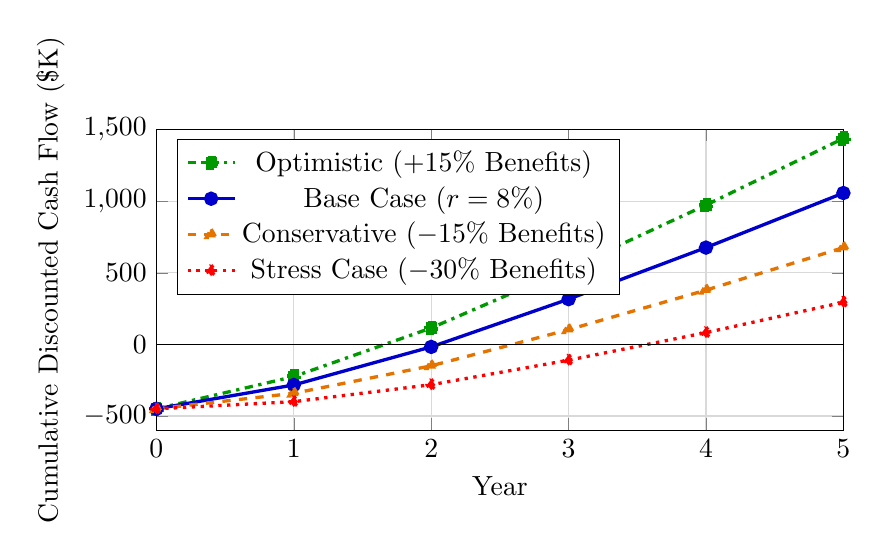
\begin{tikzpicture}
\begin{axis}[
    width=0.85\textwidth,
    height=5.4cm,
    xlabel={Year},
    ylabel={Cumulative Discounted Cash Flow (\$K)},
    xmin=0, xmax=5,
    ymin=-600, ymax=1500,
    xtick={0,1,2,3,4,5},
    grid=both,
    major grid style={gray!30},
    legend pos=north west,
    every axis plot/.append style={very thick}
]
\addplot[green!60!black, dashdotted, mark=square*] coordinates {
    (0,-450) (1,-225.0) (2,114.6) (3,529.0) (4,973.1) (5,1438.6)
};
\addlegendentry{Optimistic ($+15\%$ Benefits)}

\addplot[blue!80!black, mark=*] coordinates {
    (0,-450) (1,-283.3) (2,-17.5) (3,315.9) (4,676.1) (5,1057.2)
};
\addlegendentry{Base Case ($r=8\%$)}

\addplot[orange!90!black, dashed, mark=triangle*] coordinates {
    (0,-450) (1,-341.7) (2,-149.6) (3,102.8) (4,379.1) (5,675.8)
};
\addlegendentry{Conservative ($-15\%$ Benefits)}

\addplot[red, dotted, mark=diamond*] coordinates {
    (0,-450) (1,-400.0) (2,-281.7) (3,-110.3) (4,82.1) (5,294.3)
};
\addlegendentry{Stress Case ($-30\%$ Benefits)}

\addplot[black, thin] coordinates {(0,0) (5,0)};
\end{axis}
\end{tikzpicture}
\end{english}
\caption{תזרים מזומנים מצטבר מהוון לאורך $5$ שנים בארבעה תרחישי רגישות ($r=8\%$). גם בתרחיש קיצון של ירידה של $30\%$ בתועלות, הפרויקט מניב \textenglish{NPV} חיובי של $\$294.3\text{K}$.}
\label{fig:roi-cashflow}
\end{figure}
